\section{Riemannsummen (Riemannintegral)}
\subsection{Riemansumme}
Wir betrachten die folgende Einteilung des Intervals $[a,b]$:\[
E: [a,b] = \bigcup_{k=1}^{N}[x_{k-1}, x_k] \text{ mit } x_k = a + k \cdot \frac{b-a}{N}.
\]
\[
	\xi_k \in [x_{k-1}, x_k]
\]
Die Feinheit der Zerlegung ist:
\[
\Delta x = \frac{b-a}{N} \xrightarrow{N \to \infty} = 0
\]


\begin{minipage}{0.4\columnwidth}
	Riemannintegral mit $\xi_i = t_i$ und unsymetrischer Intervaleinteilung $E$.
\end{minipage}
\begin{minipage}{0.60\columnwidth}
	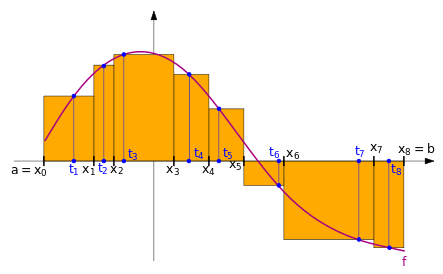
\includegraphics[scale=0.36]{riemann.png}
\end{minipage}

Somit können wir die Riemannsumme konkret berechnen:
\begin{align*}
\int_a^b f(x)\;dx &=\sum (f,E,\xi)\\
&= \lim_{N \to \infty} \underbrace{\sum_{k=1}^{N}
	\underbrace{f(\xi_k)}_{\text{``Höhe''}} \cdot \underbrace{\Delta x}_{\text{``Länge''}}}_{\text{Riemann-Summe}}\\
&= \lim_{N \to \infty} \sum_{k=0}^{N} {f(a + k\frac{b-a}{N})} \cdot \frac{b-a}{N}
\end{align*}


\subsection{Riemann Integrierbar}
\begin{definition}[Riemann integrierbar] \index{Riemann integrierbar} Die Funktion $f$ heisst auf [a, b] Riemann integrierbar, falls der Grenzwert ($I \in \R$) existiert.
\[
	\lim_{N \to \infty} = \sum_{k = 1}^N f(\xi_k) \cdot \Delta x = I \hspace{0.5cm} \text{mit } \xi_k \in [x_{k-1}, x_k]
\]
\end{definition}

\begin{definition}[Riemann integrierbar v.2] \index{Riemann integrierbar v.2}
Die Funktion $f$ heisst auf [a, b] Riemann integrierbar falls es ein $I \in \R$ gibt sodass $\forall \epsilon > 0$ gilt:
\[
	\lim_{N \to \infty} \left| \sum_{k = 1}^N f(\xi_k) \cdot \Delta x) - I \right| < \epsilon \hspace{0.5cm} \text{mit } \xi_k \in [x_{k-1}, x_k]
\]
\end{definition}
\textbf{Merke:}\\
$f$ monoton + Definitionsbereich kompakt $\Rightarrow$ $f$ ist R integrierbar\\
$f$ stetig + Definitionsbereich kompakt $\Rightarrow$ $f$ ist R integrierbar

%\subsection*{Beispiel}
%Es soll das Intergral mittels Riemannschen Summe berechnet werden: $\int_a^b
%e^{\lambda x}\,dx, \; \lambda \in \R$. $f(x) = e^{\lambda x}$

%Zuerst unterteilt man das Intervall $[a,b]$: $E: [a,b] =
%\bigcup_{k=1}^N[c_{k-1}, c_k]$ mit $c_k = a + k\cdot \frac{b-a}{N}$.

%Die Feinheit dieser Zerlegung ist somit $\delta(E) = \max\{c_k - c_{k-1} | k =
%1 \ldots N\} = \frac{b-a}{N}$. Dabei gilt $\delta(E) = \frac{b-a}{N} \to 0$ ($N
%\to \infty$). Dies ist wichtig. Wir müssen die Feinheit unglaublich klein
%bekommen können, also nahezu $0$. Je feiner die Feinheit desto genauer wird
%unsere Riemann'sche Summe. Der Grenzwert dieser Summe für $N \to \infty$ ist der
%Wert des bestimmten Riemann-Integrals.

%Zusätzlich müssen wir festlegen, an welchen Punkten in den Teilintervallen wir
%den Funktionswert auswerten. Hier legen wir fest: $x_k = c_{k-1}$, also
%jeweils am Punkt an dem das Teilintervall beginnt.

%Daraus erhalten wir nun:
%\begin{align*}
%\int_a^b e^{\lambda x}\;dx &= \lim_{N \to \infty} \underbrace{\sum_{k=0}^{N-1}
%\underbrace{f(x_k)}_{\text{``Höhe''}} \cdot
%\underbrace{\delta(E)}_{\text{``Länge''}}}_{\text{Riemann-Summe}}\\
%&= \lim_{N \to \infty} \sum_{k=0}^{N-1} \underbrace{e^{\lambda (a +
%k\frac{b-a}{N})}}_{f(x_k)} \underbrace{\frac{b-a}{N}}_{\delta(E)}\\
%&= \lim_{N \to \infty} \frac{b-a}{N} e^{\lambda a} \sum_{k=0}^{N-1}(e^{\lambda
%\frac{b-a}{N}})^k\\
%&= \lim_{N \to \infty} \frac{b-a}{N} e^{\lambda a} \frac{1-e^{\lambda
%(b-a)}}{1-e^{\lambda \frac{b-a}{N}}}
%\end{align*}

%Wir wissen, dass $\rho = \frac{b-a}{N} \to 0$ für $N \to \infty$. Somit
%ersetzten wir es entsprechend:
%\begin{align*}
%\int_a^b e^{\lambda x}\;dx &= \lim_{\rho \to 0} \rho \cdot e^{\lambda a} \cdot
%\frac{1-e^{\lambda(b-a)}}{1-e^{\lambda \rho}}\\
%&= \lim_{\rho \to 0} \frac{\rho (e^{\lambda a} - e^{\lambda b})}{1-e^{\lambda
%\rho}}\\
%&\overset{\text{d'H}}= \lim_{\rho \to 0} \frac{e^{\lambda a} - e^{\lambda
%b}}{-\lambda e^{\lambda \rho}}\\
%&= \frac{e^{\lambda a} - e^{\lambda b}}{-\lambda} = \frac{1}{\lambda}(e^{\lambda
%a} - e^{\lambda b})
%\end{align*}